\chapter{Analýza}
\section{Získanie USB packetov}
Na získavanie USB paketov nám bude obecne slúžiť paket sniffer. Väčšina paket analyzátorov má implementované vlastné sniffery a preto sme sa o to pokúsili tiež. Narazili sme ale na niekoľko zásadných problémov, ktoré sa úzko viažu s platformou na ktorú cielime s našou aplikáciou~--~Windows.

Microsoft dokumentácia podrobnejšie opisuje komunikáciu medzi HID zaridením a kernel/user-mode aplikáciou~\cite{hid_opening_collections}. Keďže naša aplikácia beží v user-mode, prejdeme si tento spôsob:
\begin{enumerate}
\item Aplikácia nájde a identifikuje HID zariadenie.
\item Aplikácia pomocou metódy \textit{CreateFile} otvorí spojenie s HID zariadením.
\item Aplikácia pomocou \textit{HID API}~\cite{hid_api} metód \textit{HidD\_Xxx} získa \textit{Preparsed Data} a informácie ohľadom HID zariadenia.
\item \textbf{Aplikácia použije metódu \textit{ReadFile} resp. \textit{WriteFile} na získanie inputu zariadenia resp. poslanie reportu zariadeniu.}
\item Aplikácia pomocou \textit{HID API}~\cite{hid_api} metód \textit{HidP\_Xxx} interpretuje HID reporty.
\end{enumerate}

\subsection{Windows exclusive mód}
Windows má definovaný tzv. \textit{Access Mode}, ktorý určuje restrikciu prístupu \textit{HID Clienta} k HID zariadeniu. 
Ten môže byť buď \textit{Shared} alebo \textit{Exclusive}. \textit{Exclusive Mode} zabraňuje ostatným \textit{HID Clientom} v zachytávaní alebo získavaní inputu HID zariadenia, pokiaľ nie sú hlavným príjemcom daného inputu. Preto z bezpečnostných dôvodov otvára \textit{RIM (Raw Input Manager)} niektoré zariadenia v \textit{Exclusive Mode}.

Ak je zariadenie otvorené v \textit{Exclusive Mode}, aplikácia má stále prístup k niektorým jeho údajom pomocou  \textit{HID API}~\cite{hid_api} metód  \textit{HidD\_\textbf{Get}Xxx}. Tieto metódy nám obecne umožnia získať niektoré descriptory zariadenia, tak ako aj jeho \textit{Preparsed Data}. Nie je nám ale umožnené volať metódu \textit{ReadFile}, takže nemáme akým spôsobom zachytávať komunikáciu HID zariadenia s clientom.

Tabuľka zariadení~\cite{hid_access} (obrázok~\ref{obr:kap3:access_mode}), ktoré \textit{RIM} otvára v \textit{Exclusive Mode} obsahuje aj tie, ktoré sme si v úvode zvolili ako podmnožinu HID zariadení na analýzu -- myš a klávesnica.

\begin{figure}[!htb]
	\centering
	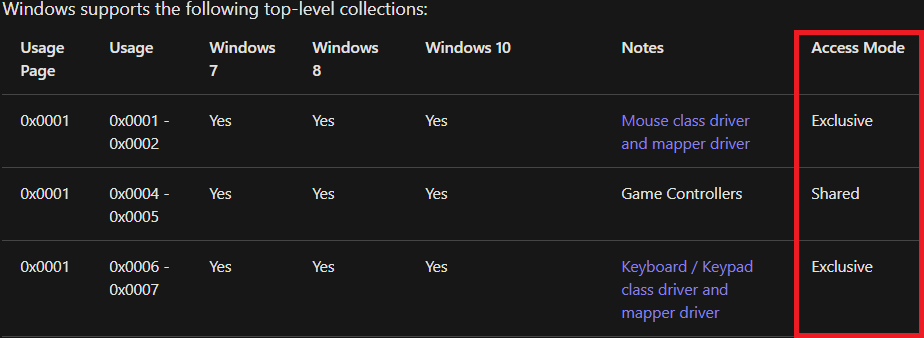
\includegraphics[width=\textwidth]{img/kap3_access_mode}
	\caption{Tabuľka zariadenía ich \textit{Access Mode}. Zariadenia postupne po riadkoch -- myš, joystick a klávesnica}
	\label{obr:kap3:access_mode}
\end{figure}

\newpage

\subsection{Známe knižnice}
opisat zakladne kniznice na sledovanie USB zbernice a preco som ich nemohol pouzit : libUSB, hidAPI

\subsection{Driver}
TU povedat riesenie - pouzitie driveru na komunikaciu so zariadenim. Existujuce windows drivery -- moufiltr, Kbdfiltr - nefunguju pre USB

TU spomenut posledne mozne riesenie - napisanie vlastneho filter driveru. 

\subsection{Third-party aplikácie}
opisat odkial nakoniec ziskavam packety - USBPcap a Wireshark









\section{Spracovávanie pcap súborov}
moznosti ako citat pcap subory : bud pouzit uz existujucu kniznicu : na linuxe Libpcap, windows NPcap(deprecated WinPcap), alebo citat subory manualne : std::istream alebo QFile
\section{Sémantická reprezentácia dát}
ako si z dat vytiahnut udaje ktore su potom pouzite na semanticku analyzu implementovanych HID zariadeni : HID Report parser, InputValues a EndpointDevice struct.
Nasledne sparovanie - ako vybrat spravny report pre konkretny input
\section{Voľba frameworku}
obecne co by som od toho GUI priblizne chcel, potom opisat preco som si vybral prave Qt a v nasledujucich kapitolach opisat rozhodnutia uz v Qt
dovod preco som si zvolil qt namiesto inych c++ GUI frameworkov(napriklad sfml)
\section{Zobrazenie základných informácií}
ako zobrazovat zakladne info o packete : pouzit QListWidget alebo QTableWidget (pripadne nieco ine ako nejaky abstract viewmodel), narok na zakladne funkcionality : lahka rozsiritenlnost o dalsie ''stlpceky'' , moznost jednoduchej interakcie(doubleClick na polozku). Mat vsetky info na jednom okne / mat pop-up okna.
\section{Zobrazenie sémantického významu dát}
ako vyzobrazit semanticky vyznam roznych dat - descriptory, usb header, vyznam input dat roznych HID zariadeni
\section{Hexdump}
ako v qt urobit hexdump - do coho zobrazovat data(vytvorit si vlastny viewer dedeny od QAbstractScrollArea, pripadne niecoho ineho) vs najst nieco co uz v qt je a upravit to aby to sedelo poziadavkam. Vziat do uvahy bezne funkcie hexdumpu : selection mody(oznacit naraz hexa a im odpovedajuce printable), logicke oddelenie dat(napriklad farbami)








